Aquí se presenta una pequeña descripción de cómo se usa la aplicación. Este texto de ayuda se puede ver también desde la propia aplicación accediendo al menú en la ventana principal. Se encuentra tanto en español como inglés, al igual que todos los diálogos y texto de los botones. Es el propio sistema Android, en base al idioma seleccionado por defecto en el sistema operativo, el que selecciona el idioma a mostrar. En caso de no disponer del idioma correspondiente al del sistema, por defecto se mostrarán los textos en inglés.
\section{Página de ayuda de VNC++}
\subsection{Manejo principal}
Para crear una nueva conexión pulse el icono ``+'' en la barra superior de Acción (Ver Figura A.1). Una vez dentro, es necesario especificar la IP del servidor, así como un nombre de identificación de la conexión. El puerto por defecto es el 5900, pudiéndose cambiar, así como la contraseña, pudiéndose dejar en blanco si no se necesita.
\begin{figure}[h]
\hfill
\begin{minipage}[t]{.45\textwidth}
\begin{center}
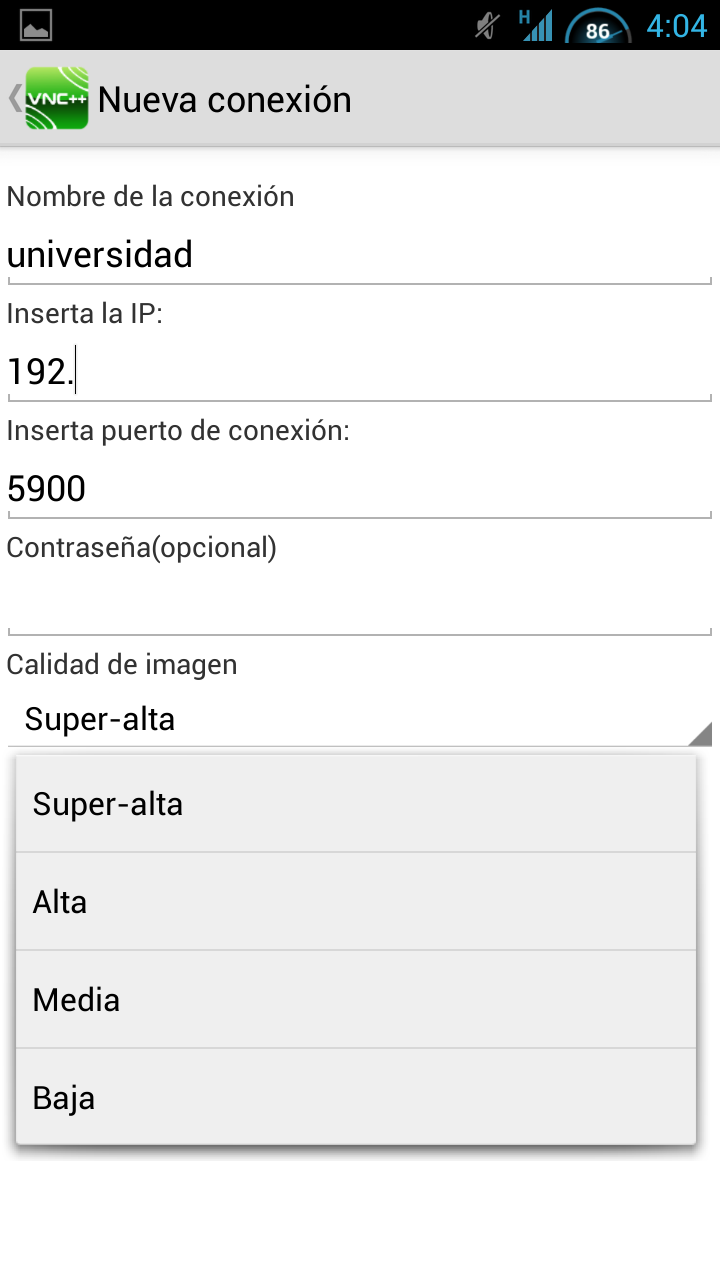
\includegraphics[scale=0.19]{Screenshot_2013-06-14-04-04-46.png}
\caption{Nueva conexión}
\end{center}
\end{minipage}
\hfill
\begin{minipage}[t]{.45\textwidth}
\begin{center}
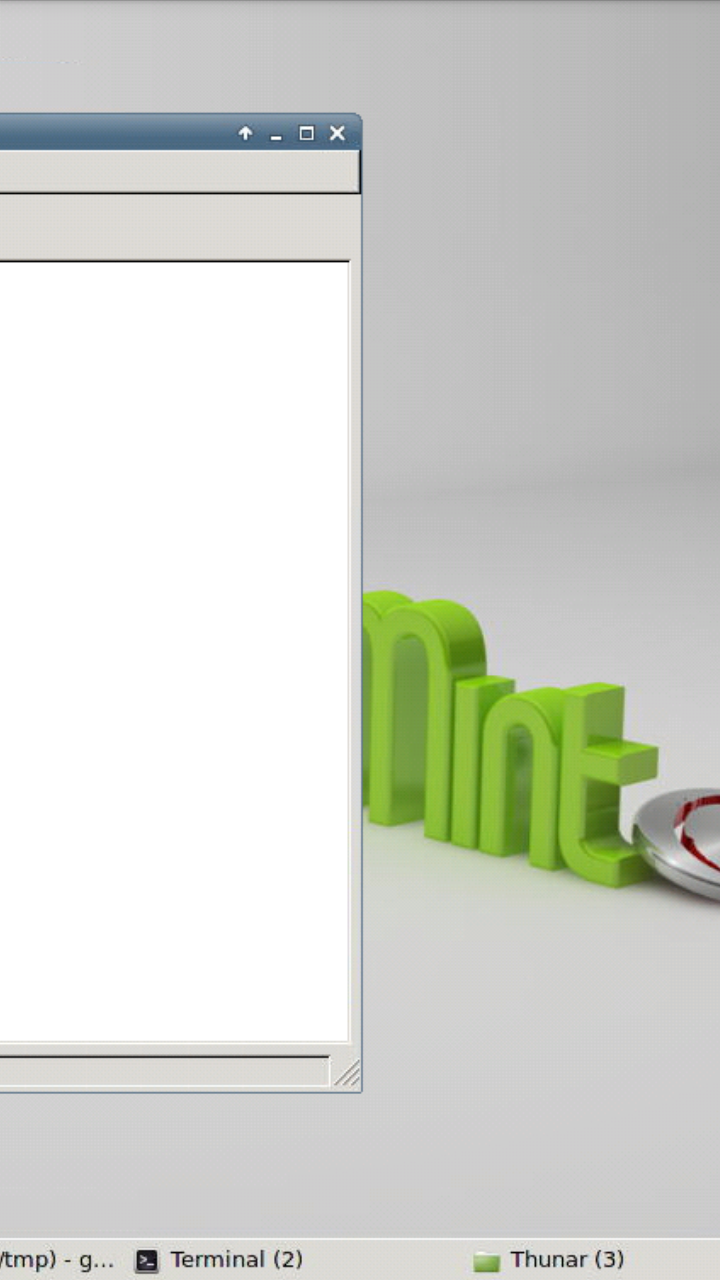
\includegraphics[scale=0.19]{Screenshot_2013-06-19-16-37-43.png}
\caption{Vista del escritorio}
\end{center}
\end{minipage}
\hfill
\end{figure}
\newpage

El desplegable de calidades sirve para indicar la calidad de la imagen. Se puede elegir entre calidad super-alta, alta, media o baja, según el tipo de conexión del usuario ya sea más lenta o rápida, o simplemente por necesidad de cierta calidad de imagen.\\

En el botón desplegable de opciones en la actividad principal se puede acceder a tres submenús:
\begin{itemize}
\item La opción de Configuración: permite, a través de dos switches de selección, marcar si se recuerda o no la opción de confirmar salida, así como ocultar el cursor o no (Ver Figura A.3).
\item Manual de uso parecido al que se está narrando (Ver Figura A.4).
\item Sección ``Acerca de'' donde se reflejan los creadores de la aplicación, así como el tipo de licencia y las librerías usadas (Ver Figura A.8).
\end{itemize}

\begin{figure}[h]
\hfill
\begin{minipage}[t]{.45\textwidth}
\begin{center}
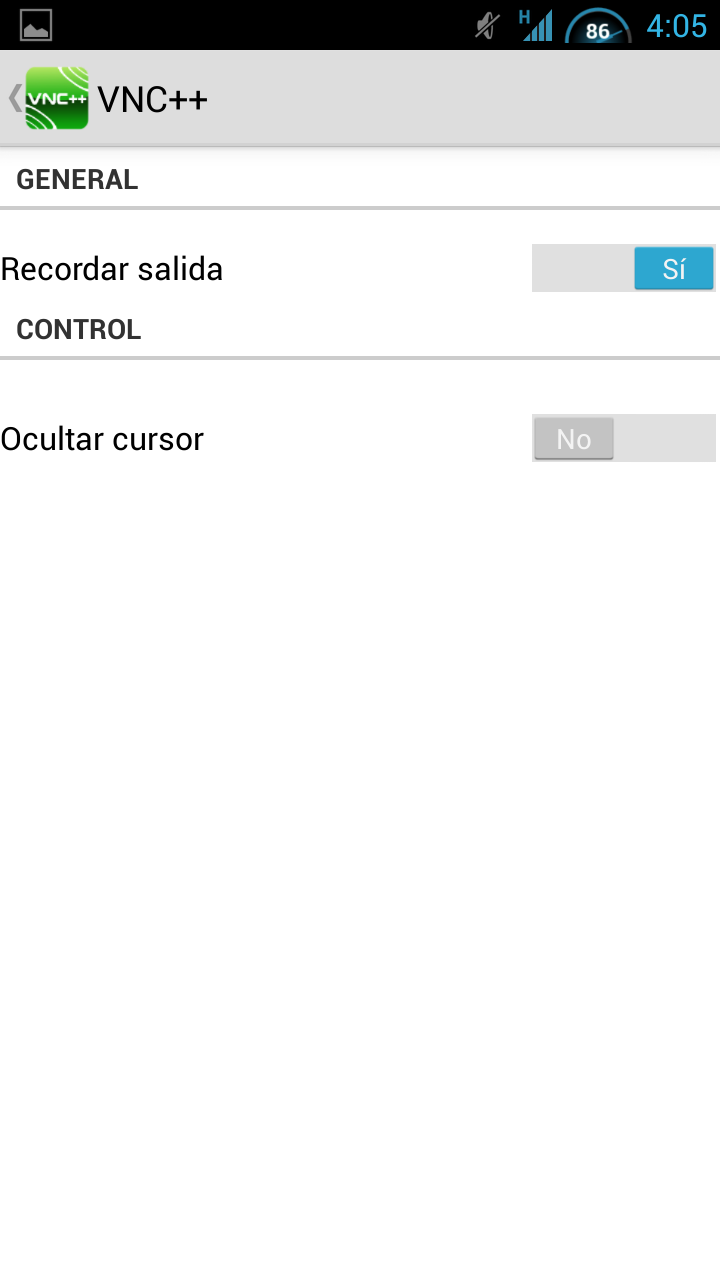
\includegraphics[scale=0.2]{Screenshot_2013-06-14-04-05-03.png}
\caption{Configuración}
\end{center}
\end{minipage}
\hfill
\begin{minipage}[t]{.45\textwidth}
\begin{center}
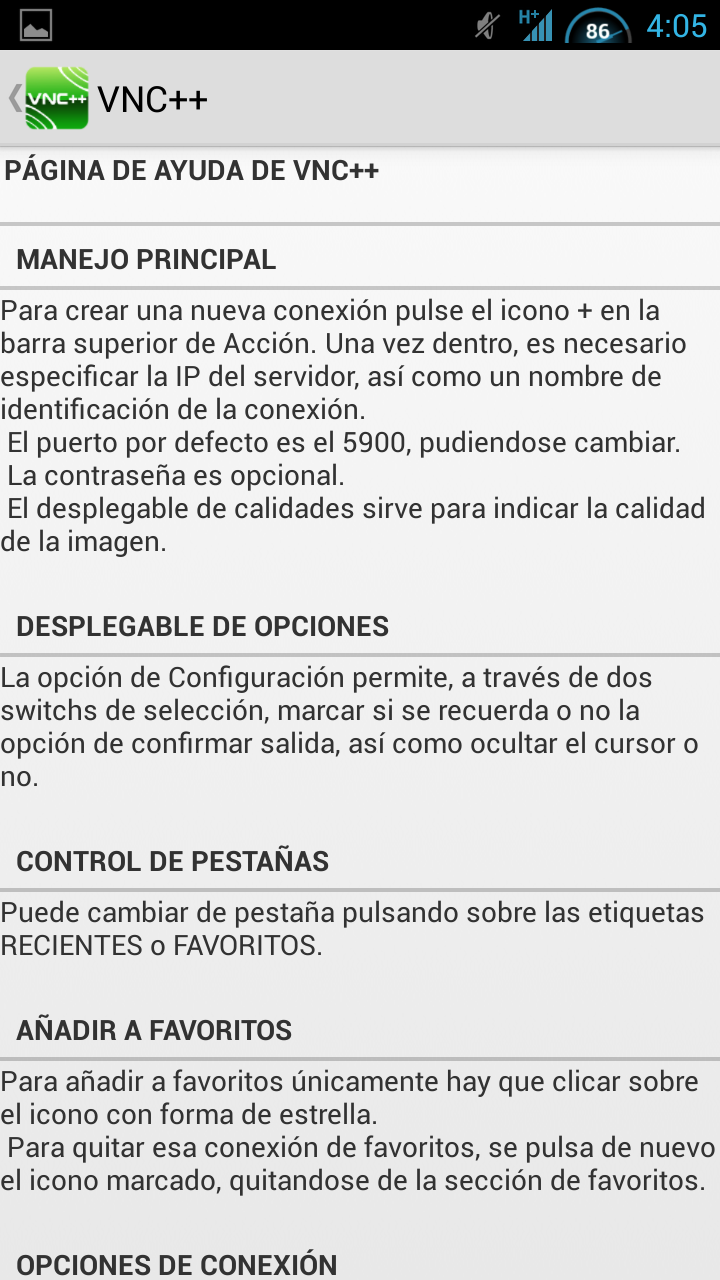
\includegraphics[scale=0.2]{Screenshot_2013-06-14-04-05-52.png}
\caption{Manual de uso}
\end{center}
\end{minipage}
\hfill
\end{figure}

\subsection{Control de pestañas}
Se puede cambiar de pestaña pulsando sobre las etiquetas RECIENTES o FAVORITOS, y así ver las distintas conexiones creadas (Ver Figura A.5).
\subsection{Añadir a favoritos}
Para añadir a favoritos únicamente hay que clicar sobre el icono con forma de estrella (Ver Figura A.5).\\

Para quitar esa conexión de favoritos, se pulsa de nuevo el icono marcado, quitándose de la sección de favoritos.
\subsection{Opciones de conexión}
Al pulsar sobre una conexión de la lista, se presenta un menú de opciones. Desde ahí se puede conectar, mostrar la información de la conexión, editar y eliminar dicha conexión. También se puede conectar pulsando el icono de la derecha con forma de flecha.

\subsection{Opciones de edición}
Se podrá modificar cualquier valor previo de la conexión, a excepción del identificador elegido, del mismo modo que se crea una nueva conexión.
\subsection{Menú lateral}
Una vez cargada la imagen se puede acceder al menú de opciones, tanto desde el botón físico del terminal, como arrastrando desde la izquierda de la pantalla para sacar el menú lateral. Una vez ahí se puede mostrar teclado, mandar teclas, centrar imagen, mostrar una ayuda reducida  y desconectar (Ver Figura A.6).
\begin{figure}[h]
\hfill
\begin{minipage}[t]{.45\textwidth}
\begin{center}
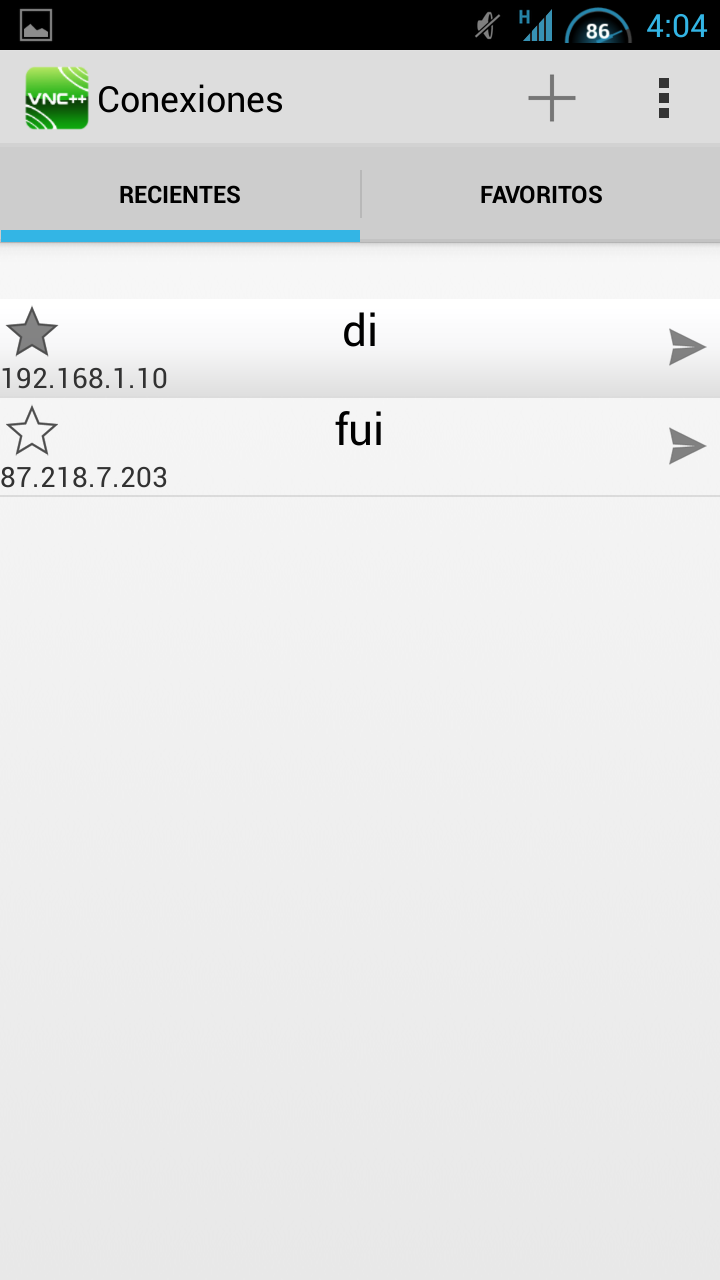
\includegraphics[scale=0.2]{Screenshot_2013-06-14-04-04-09.png}
\caption{Pestañas}
\end{center}
\end{minipage}
\hfill
\begin{minipage}[t]{.45\textwidth}
\begin{center}
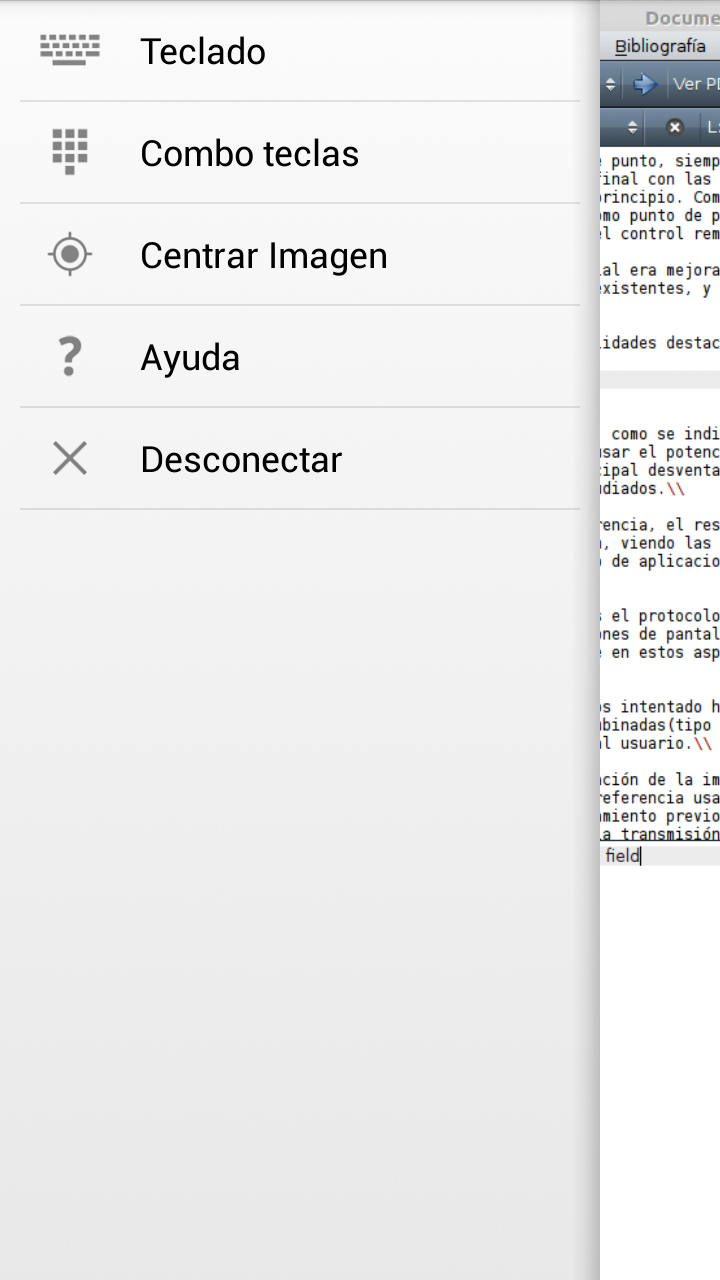
\includegraphics[scale=0.2]{Screenshot_2013-06-14-04-03-02.png}
\caption{Menú lateral}
\end{center}
\end{minipage}
\hfill
\end{figure}
\subsection{Manejo}
Para mandar evento click, simplemente haga una pulsación con el dedo.\\

Para hacer click derecho, mantenga presionado el dedo sobre la pantalla durante unos 3 segundos.\\

Para hacer zoom, coloque un dedo sobre la pantalla, mientras con otro dedo aleje o acerque del primer dedo, a modo de pinza.
\subsection{Envío de teclas especiales}
Para mandar eventos ctrl, alt, supr, shift, basta con seleccionar la tecla ``Combo teclas'', y en la ventana emergente seleccionar las teclas que se quieran enviar (Ver Figura A.7).
\begin{figure}[h]
\hfill
\begin{minipage}[t]{.45\textwidth}
\begin{center}
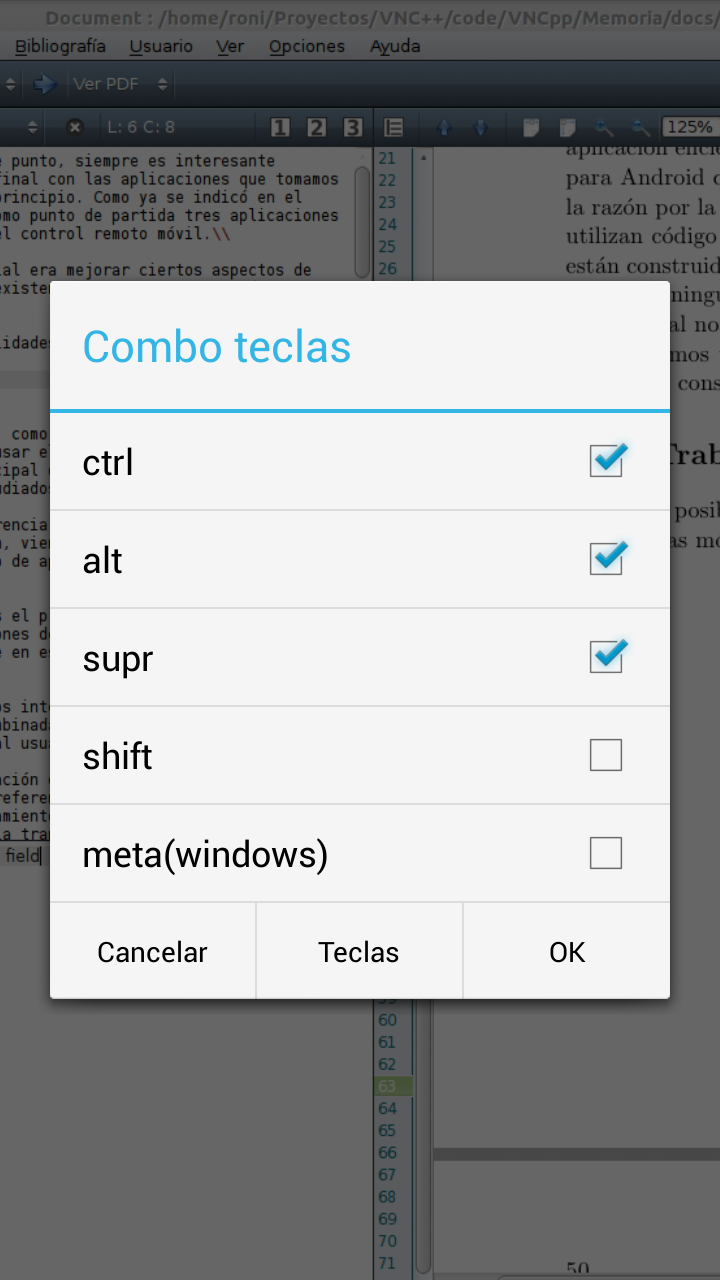
\includegraphics[scale=0.2]{Screenshot_2013-06-14-04-03-19.png}
\caption{Teclas especiales}
\end{center}
\end{minipage}
\hfill
\begin{minipage}[t]{.45\textwidth}
\begin{center}
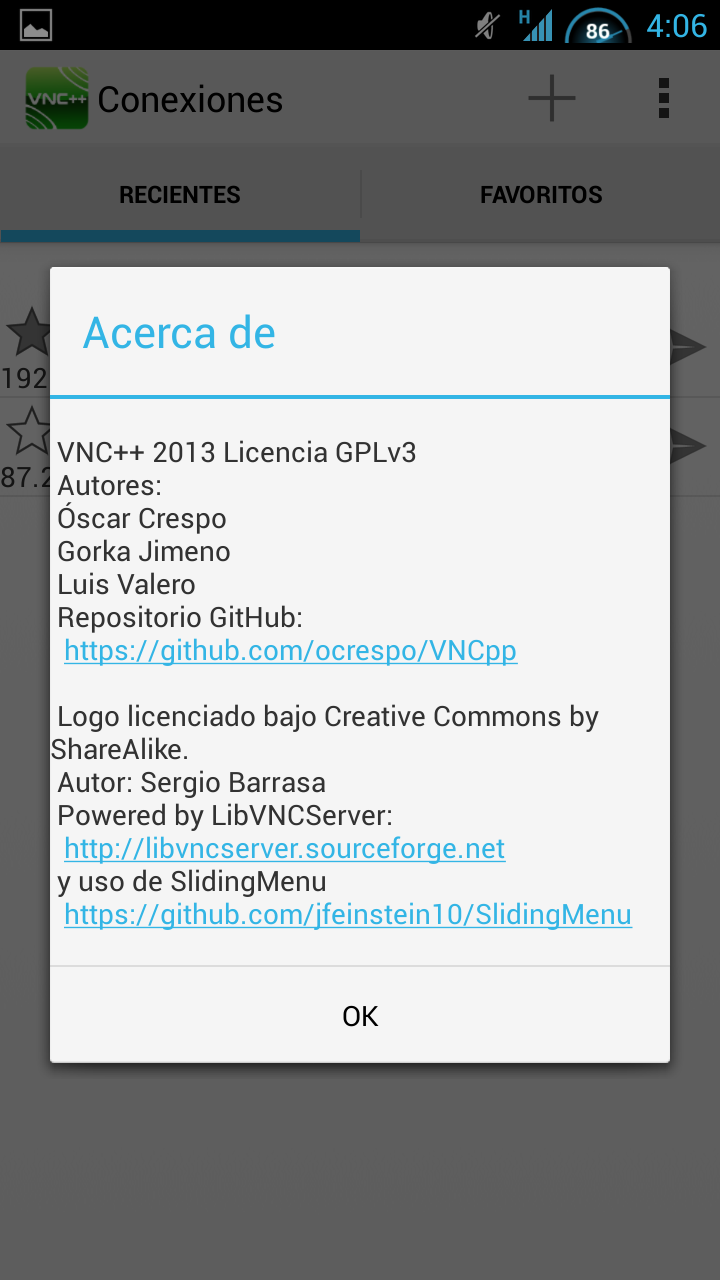
\includegraphics[scale=0.2]{Screenshot_2013-06-14-04-06-07.png}
\caption{Acerca de}
\end{center}
\end{minipage}
\hfill
\end{figure}

Las teclas función (F1, F2, etc) y el resto de letras, se pueden seleccionar desde el botón central ``Teclas''.
